\documentclass{article}
\usepackage[utf8]{inputenc}
\usepackage{polski}
\usepackage{fancyhdr} % Required for custom headers
\usepackage{lastpage} % Required to determine the last page for the footer
\usepackage{extramarks} % Required for headers and footers
\usepackage[usenames,dvipsnames]{color} % Required for custom colors
\usepackage{graphicx} % Required to insert images
\usepackage{listings} % Required for insertion of code
\usepackage{courier} % Required for the courier font
\usepackage[onelanguage]{algorithm2e}
\usepackage{pgfplots}
\pgfplotsset{width=10cm,compat=1.9}
\usepgfplotslibrary{external}
\usepackage{enumerate}
% Margins
\topmargin=-0.45in
\evensidemargin=0in
\oddsidemargin=0in
\textwidth=6.5in
\textheight=9.0in
\headsep=0.25in
\usepackage{tikz}
\usetikzlibrary{calc}
\linespread{1.1} % Line spacing

% Set up the header and footer
\pagestyle{fancy}
\lhead{\hmwkAuthorName} % Top left header
\chead{\hmwkClass\ \hmwkTitle} % Top center head
\rhead{\firstxmark} % Top right header
\lfoot{\lastxmark} % Bottom left footer
\cfoot{} % Bottom center footer
\rfoot{Strona\ \thepage\ z\ \protect\pageref{LastPage}} % Bottom right footer
\renewcommand\headrulewidth{0.4pt} % Size of the header rule
\renewcommand\footrulewidth{0.4pt} % Size of the footer rule

\setlength\parindent{0pt} % Removes all indentation from paragraphs
%----------------------------------------------------------------------------------------
%	DOCUMENT STRUCTURE COMMANDS
%	Skip this unless you know what you're doing
%----------------------------------------------------------------------------------------

% Header and footer for when a page split occurs within a problem environment
\newcommand{\enterProblemHeader}[1]{
}

% Header and footer for when a page split occurs between problem environments
\newcommand{\exitProblemHeader}[1]{
\nobreak\extramarks{#1 (continued)}{#1 continued on next page\ldots}\nobreak
\nobreak\extramarks{#1}{}\nobreak
}

\setcounter{secnumdepth}{0} % Removes default section numbers
\newcounter{homeworkProblemCounter} % Creates a counter to keep track of the number of problems

\newcommand{\homeworkProblemName}{}
\newenvironment{homeworkProblem}[1][Zadanie \arabic{homeworkProblemCounter}]{ % Makes a new environment called homeworkProblem which takes 1 argument (custom name) but the default is "Problem #"
\stepcounter{homeworkProblemCounter} % Increase counter for number of problems
\renewcommand{\homeworkProblemName}{#1} % Assign \homeworkProblemName the name of the problem
\section{\homeworkProblemName} % Make a section in the document with the custom problem count
\enterProblemHeader{\homeworkProblemName} % Header and footer within the environment
}{
\exitProblemHeader{\homeworkProblemName} % Header and footer after the environment
}

\newcommand{\problemAnswer}[1]{ % Defines the problem answer command with the content as the only argument
\noindent\framebox[\columnwidth][c]{\begin{minipage}{0.98\columnwidth}#1\end{minipage}} % Makes the box around the problem answer and puts the content inside
}

\newcommand{\homeworkSectionName}{}
\newenvironment{homeworkSection}[1]{ % New environment for sections within homework problems, takes 1 argument - the name of the section
\renewcommand{\homeworkSectionName}{#1} % Assign \homeworkSectionName to the name of the section from the environment argument
\subsection{\homeworkSectionName} % Make a subsection with the custom name of the subsection
\enterProblemHeader{\homeworkProblemName\ [\homeworkSectionName]} % Header and footer within the environment
}{
\enterProblemHeader{\homeworkProblemName} % Header and footer after the environment
}

%----------------------------------------------------------------------------------------
%	NAME AND CLASS SECTION
%----------------------------------------------------------------------------------------

\newcommand{\hmwkTitle}{Lista nr 5} % Assignment title
\newcommand{\hmwkDueDate}{Środa, 3 stycznia 2018} % Due date
\newcommand{\hmwkClass}{OBLICZENIA NAUKOWE} % Course/class
\newcommand{\hmwkAuthorName}{Tymoteusz Surynt} % Your name
\renewcommand*\contentsname{Podsumowanie}

%----------------------------------------------------------------------------------------
%	TITLE PAGE
%----------------------------------------------------------------------------------------

\title{
\vspace{2in}
\textmd{\textbf{\hmwkClass:\ \hmwkTitle}}\\
\normalsize\vspace{0.1in}\small{\hmwkDueDate}\\
\vspace{3in}
}

\author{\textbf{\hmwkAuthorName}}
\date{Numer indeksu: 229794} % Insert date here if you want it to appear below your name

%----------------------------------------------------------------------------------------

\begin{document}

\maketitle

%----------------------------------------------------------------------------------------
%	TABLE OF CONTENTS
%----------------------------------------------------------------------------------------

%\setcounter{tocdepth}{1} % Uncomment this line if you don't want subsections listed in the ToC

\newpage
\tableofcontents
\newpage
%----------------------------------------------------------------------------------------
%	Structure
%----------------------------------------------------------------------------------------

% To have just one problem per page, simply put a \clearpage after each problem

\begin{homeworkProblem}
%opis problemu
\subsection{Opis problemu}
Stworzenie modułu, dzięki któremu będzie można skorzystać ze struktury, która pozwoli efektywnie prowadzić obliczenia na blokowej macierzy A z dużą ilością elementów (e.g. $10000 \times 10000$, $50000 \times 50000$)
%opis rozwiązania
\subsection{Opis rozwiązania}
Na początku warto zauważyć, że macierz A jest wstęgową macierzą blokową. Z tego faktu wiemy, że niezerowe wartości znajdują się na przekątnej i zaraz obok przekątnej macierzy. Łatwo też da się zauważyć, że maksymalna liczba niezerowych bloków macierzy w jednym wierszu wynosi 3. Mając taką wiedzę można łatwo zbudować tablicę, która w każdej komórce będzie pamiętać 3 bloki z wartościami. Łatwo zauważyć, że w pierwszej i ostatniej komórce powinny być tylko 2 bloki, ale tę niedogodność łatwo obejść przez inicjonowanie komórek 1 i 3 (B i C) jako zera. \\
Każdy blok zapamiętywany w tablicy ma swoje właściwości pozwalające mu zapamiętać tylko najważniejsze dane:
\begin{enumerate}
\item komórka zapamiętująca blok $B_k$. Jest ona macierzą o wysokości l (wielkość pojedynczego bloku) oraz o szerokości 2. Taka konstrukcja wynika z faktu, że tylko dwie ostatnie wartości w tym bloku mogą mieć inne wartości niż 0, więc nie ma sensu pamiętania wszystkich
\item komórka zapamiętująca blok $A_k$. Jest ona macierzą $l \times l$. Niestety w tym bloku każda wartość może być niezerowa i na całości bloku będą prawdopodobnie prowadzone obliczenia dlatego nie ma dużego zysku w próbie optymalizacji miejsca zajmowanego przez ten blok
\item komórka zapamiętująca blok $C_k$. Jest ona macierzą $l \times l$ wypełnioną na początku samymi zerami. Tutaj celowo nie optymalizuje miejsca zajmowanego przez macierz, mimo że wartości niezerowe znajdują się tylko na przekątnej macierzy. Takie działanie wynika z faktu, że przy liczeniu eliminacji Gaussa z i bez częściowego wyboru elementu głównego korzystam z pozostałych komórek do obliczeń
\item przy obliczaniu wektora metodą eliminacji Gaussa z częściowym wyborem elementu głównego występuje tymczasowa komórka, w której zapisywane są odpowiednie liczby w razie, gdyby nastąpiła zamiana wiersza między blokami
\end{enumerate}

Funkcje wchodzące w skład modułu blocksys wraz z krótkim opisem i przykładami użycia:
\begin{itemize}
\item $importMatrix(fileLocation)$\\
funkcja odpowiedzialna za importowanie macierzy z pliku. Jej jedynym parametrem jest ścieżka do pliku. Funkcja zwraca rozmiar całej macierzy $n$, rozmiar pojedynczego bloku $l$ oraz samą tablicę reprezentującą macierz blokową $A$ w postaci opisanej powyżej.\\
Przykład użycia:
$$result=importMatrix("/home/user/Desktop/ON/Dane16\_1\_1/A.txt")$$
\item $getError(x, value::Float64, n::Int64)$\\
funkcja odpowiedzialna za wyliczanie średniego błędu bezwzględnego wektora, jeśli każda jego wartość powinna przyjmować jedną wartość(e.g. 1.0). Funkcja jako parametry przyjmuje wektor x, wartość jaką powinny przyjmować komórki wektora ($value$) oraz wielkość wektora $n$, natomiast zwraca wartość w typie Float64 reprezentującą średni błąd bezwzględny.\\
Przykład użycia:
$$err=getError(x,1.0,16)$$
\item $exportVectorNoError(fileLocation, x)$\\
funkcja odpowiedzialna za eksportowanie wektora do zadanego pliku bez podawania błędu na początku pliku. Funkcja jako parametry przyjmuje ścieżkę do pliku oraz wektor, który chcemy zapisać\\
Przykład użycia:
$$exportVectorNoError("/home/user/Desktop/ON/Tests/x.txt",x)$$
\item $exportVectorError(fileLocation, x, err)$\\
funkcja odpowiedzialna za eksportowanie wektora do zadanego pliku z podaniem na początku pliku błędu. Funkcja jako parametry przyjmuje ścieżkę do pliku, wektor oraz błąd. \\
Przykład użycia:
$$exportVectorNoError("/home/user/Desktop/ON/Tests/x.txt",x,err)$$
\item $importVector(fileLocation)$\\
funkcja odpowiedzialna za importowanie wektora z pliku. Jej jedynym parametrem jest ścieżka do pliku. Funkcja zwraca rozmiar wektora $n$ oraz wektor w postaci tablicy z elementami typu Float64.\\
Przykład użycia:
$$b=importVector("/home/user/Desktop/ON/Dane16\_1\_1/b.txt")$$
\item $printfMatrix(A,b, l::Int64, n::Int64)$
funkcja odpowiedzialna za wyświetlanie komórek tablicy, omówionej na samym początku tego zagadnienia. Wyświetla tylko komórki w których potencjalnie mogą być niezerowe wartości. Funkcja przyjmuje jako parametry macierz $A$, wektor $b$, wielkość pojedynczego bloku oraz wielkość całej macierzy.\\
Przykład użycia:
$$printfMatrix(A,b, 4, 16)$$
\item $printfMatrix2(A,b, l::Int64, n::Int64)$\\
funkcja odpowiedzialna za wyświetlanie komórek tablicy, omówionej na samym początku tego zagadnienia z dodatkowym 4 blokiem występującym przy korzystaniu z eliminacji Gaussa z częściowym wyborem elementu głównego. Wyświetla tylko komórki w których potencjalnie mogą być niezerowe wartości. Funkcja przyjmuje jako parametry macierz $A$, wektor $b$, wielkość pojedynczego bloku oraz wielkość całej macierzy.\\
Przykład użycia:
$$printfMatrix2(A,b, 4, 16)$$
\item $gaussElimination(n::Int64,l::Int64,AB,v)$\\
funkcja odpowiedzialna za wyliczenie wektora $x$ metodą eliminacji Gaussa bez wyboru elementu głównego. Funkcja jako parametry przyjmuje wielkość macierzy $A$, długość pojedynczego bloku, macierz $A$ w postacie opisanej na początku tego podpunktu oraz wektor $b$ (w tym przypadku nazywa się $v$, później w miarę obliczeń zmieni nazwę na właściwą, czyli $b$). Funkcja zwraca jako wynik czwórkę, której pierwszą składową jest nowa macierz $A$ będąca wynikiem pierwszej części eliminacji Gaussa, druga składowa to nowy wektor $b$, który również powstał przez eliminację Gaussa, trzecia składowa to wektor $x$, natomiast ostatnia składowa przyjmuje wartość 0, jeśli obliczanie przeszło bez większego problemu oraz wartość 1, jeśli element na przekątnej był zbliżony do 0.
\\
Przykład użycia:
$$w=gaussElimination(16,4,A,b)$$
\item $gaussElimination2(n::Int64,l::Int64,AB,v)$\\
funkcja odpowiedzialna za wyliczenie wektora $x$ metodą eliminacji Gaussa z wyborem elementu głównego. Funkcja jako parametry przyjmuje wielkość macierzy $A$, długość pojedynczego bloku, macierz $A$ w postacie opisanej na początku tego podpunktu z dodatkowym blokiem na obliczenia w każdym wierszu oraz wektor $b$ (w tym przypadku nazywa się $v$, później w miarę obliczeń zmieni nazwę na właściwą, czyli $b$). Funkcja zwraca jako wynik czwórkę, której pierwszą składową jest nowa macierz $A$ będąca wynikiem pierwszej części eliminacji Gaussa, druga składowa to nowy wektor $b$, który również powstał przez eliminację Gaussa, trzecia składowa to wektor $x$, natomiast ostatnia składowa przyjmuje wartość 0, jeśli obliczanie przeszło bez większego problemu oraz wartość 1, jeśli element na przekątnej był zbliżony do 0.
\\
Przykład użycia:
$$w=gaussElimination(16,4,A,b)$$

\end{itemize}

%wyniki
\subsection{Testy}
Testowanie obu eliminacji Gaussa będzie omawiane przy następnym zadaniu, w tym podpunkcie są przedstawione testy pozostałych funkcji. Aby przetestować powyższe funkcje posłużyłem się danymi przykładowymi, które można znaleźć na stronie pana prof. Zielińskiego ($http://cs.pwr.edu.pl/zielinski/$) w zakładce obliczenia naukowe, lista nr 5. Do uzyskania czasu posłużyłem się programem linuxowym time.\\
\begin{itemize}
\item Importowanie macierzy:\\
Czas dla 16 elementów:\\
\\
\begin{tabular}{l | r}
real & 0m 0.396s\\ \hline
user & 0m 0.354s\\ \hline
sys & 0m 0.040s\\
\end{tabular}
\\
\\Czas dla 10000 elementów:\\
\\
\begin{tabular}{l | r}
real & 0m 0.457s\\ \hline
user & 0m 0.417s\\ \hline
sys & 0m 0.038s\\
\end{tabular}
\\
\\Czas dla 50000 elementów:\\
\\
\begin{tabular}{l | r}
real & 0m 0.848s\\ \hline
user & 0m 0.818s\\ \hline
sys & 0m 0.054s\\

\end{tabular}\\
\\Poprawność importowanych danych będzie testowana przy użyciu funkcji $printfMatrix$.
\item Importowanie wektora:\\
Czas dla 16 elementów:\\
\\
\begin{tabular}{l | r}
real & 0m 0.357s\\ \hline
user & 0m 0.316s\\ \hline
sys & 0m 0.039s\\
\end{tabular}
\\
\\Czas dla 10000 elementów:\\
\\
\begin{tabular}{l | r}
real & 0m 0.360s\\ \hline
user & 0m 0.323s\\ \hline
sys & 0m 0.036s\\
\end{tabular}
\\
\\Czas dla 50000 elementów:\\
\\
\begin{tabular}{l | r}
real & 0m 0.369s\\ \hline
user & 0m 0.340s\\ \hline
sys & 0m 0.026s\\
\end{tabular}\\
\\Poprawność importowanych danych będzie testowana przy użyciu funkcji $printfMatrix$.


\item Wyświetlanie macierzy:\\
Przykład dla 16 elementów:\\
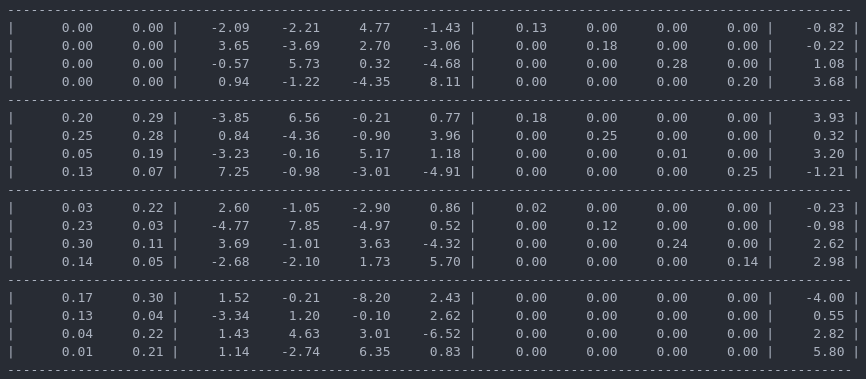
\includegraphics[scale=0.5]{printfM.png}\\
Czas dla 16 elementów:\\
\\
\begin{tabular}{l | r}
real & 0m 0.610s\\ \hline
user & 0m 0.565s\\ \hline
sys & 0m 0.040s\\
\end{tabular}
\\
\\Czas dla 10000 elementów:\\
\\
\begin{tabular}{l | r}
real & 0m 2.420s\\ \hline
user & 0m 1.346s\\ \hline
sys & 0m 1.058s\\
\end{tabular}
\\
\\Czas dla 50000 elementów:\\
\\
\begin{tabular}{l | r}
real & 0m 9.229s\\ \hline
user & 0m 4.048s\\ \hline
sys & 0m 5.127s\\
\end{tabular}\\
\\Dla przykładów z 10000 i 50000 nie ma obrazka, gdyż zajął by on dużo miejsca i byłby nieczytelny. Nie zmienia to jednak faktu, że wartości zgadzają się z tymi znajdującymi się w plikach. Warto również zauważyć, że czas jest podany razem z czasem potrzebnym na wczytanie wektora oraz macierzy, aby uzyskać czas samego wyświetlania można odjąć podane czas i te znajdujące się wyżej. 
\end{itemize}
\end{homeworkProblem}
\clearpage

%----------------------------------------------------------------------------------------
%	PROBLEM 1
%----------------------------------------------------------------------------------------

% To have just one problem per page, simply put a \clearpage after each problem

\begin{homeworkProblem}
%opis problemu
\subsection{Opis problemu}
Zadanie polegało na stworzeniu algorytmu, który efektywnie liczy metodą eliminacji Gaussa wektor x z równania $Ax=b$:
\begin{enumerate}[a)]
\item  bez wyboru elementu głównego
\item z wyborem elementu głównego
\end{enumerate}
%opis rozwiązania
\subsection{Eliminacja Gaussa bez wyboru elementu głównego:}

\begin{algorithm}[H]
 \SetKwInput{KwData}{Dane}
 \KwData{
 \\n - wielkość macierzy A\\
 l -  wielkość pojedynczego bloku\\
 AB - macierz A\\
 v - wektor b\\
 }
 \SetKwInput{KwResult}{Wynik}
 \KwResult{
	(A,b,x,$0|1$) – co zwracają składowe wyniku zostało wyjaśnione na stronie 4.\\
 }
 \SetKwInput{TitleOfAlgo}{Funkcja}
 \TitleOfAlgo{gaussElimination(n::Int64,l::Int64,AB,v)}
	$A \leftarrow deepcopy(AB)$\;
        $b \leftarrow deepcopy(v)$\;
       $X \leftarrow Array{Float64}(n)$\;
        \For{i in 1:(l-1)}{
            \For{j in (i+1):l}{
                \If{$abs(A[1,2][i,i]) <\epsilon$}{
                    \KwRet {(A,b,X,1)}
                }
                $m \leftarrow A[1,2][j,i]/A[1,2][i,i]$\;
                \For{k in i:l}{
                    $A[1,2][j,k] \leftarrow A[1,2][j,k]-m*A[1,2][i,k]$\;
                }
                \For{k in 1:l}{
                    $A[1,3][j,k] \leftarrow A[1,3][j,k]-m*A[1,3][i,k]$\;
                }
                $b[j] \leftarrow b[j]-m*b[i]$\;
            }
        }
\end{algorithm}
\begin{algorithm}[H]
        \For{x in $2:(n/l-1)$}{
            \For{j in 1: l}{
                \If{$abs(A[x-1,2][l-1,l-1]) < \epsilon$}{
                    \KwRet{(A,b,X,1)}
                }
                $m \leftarrow A[x,1][j,1]/A[x-1,2][l-1,l-1]$\;
                $A[x,1][j,2] \leftarrow A[x,1][j,2]-m*A[x-1,2][l-1,l]$\;
                $A[x,1][j,1] \leftarrow A[x,1][j,1]-m*A[x-1,2][l-1,l-1]$\;
                \For{k in 1:l}{
                    $A[x,2][j,k] \leftarrow A[x,2][j,k]-m*A[x-1,3][l-1,k]$\;
                }
                $b[(x-1)*l+j] \leftarrow b[(x-1)*l+j]-m*b[(x-2)*l+l-1]$\;
            }
        


            \For{j in 1: l}{
                \If {$abs(A[x-1,2][l,l]) < \epsilon$}{
                    \KwRet{(A,b,X,1)}
                }
                $m \leftarrow A[x,1][j,2]/A[x-1,2][l,l]$\;
                $A[x,1][j,2] \leftarrow A[x,1][j,2]-m*A[x-1,2][l,l]$\;
                \For{k in 1:l}{
                    $A[x,2][j,k] \leftarrow A[x,2][j,k]-m*A[x-1,3][l,k]$\;
                }
                $b[(x-1)*l+j] \leftarrow b[(x-1)*l+j]-m*b[(x-2)*l+l]$\;
            }
            \For{i in 1:(l-1)}{
                \For {j in (i+1):l}{
                    \If {$abs(A[x,2][i,i]) < \epsilon$}{
                        \KwRet{(A,b,X,1)}
                    }
                    $m \leftarrow A[x,2][j,i]/A[x,2][i,i]$\;
                    \For {k in i:l}{
                        $A[x,2][j,k] \leftarrow A[x,2][j,k]-m*A[x,2][i,k]$\;
                    }
                    \For {k in 1:l}{
                        $A[x,3][j,k] \leftarrow A[x,3][j,k]-m*A[x,3][i,k]$\;
                    }
                    $b[(x-1)*l+j] \leftarrow b[(x-1)*l+j]-m*b[(x-1)*l+i]$\;
                }
                
            }
        }
        
    \end{algorithm}
    \newpage
\begin{algorithm}[H]
        \For {j in 1: l}{
            \If {$abs(A[n/l-1,2][l-1,l-1]) < \epsilon$}{
                \KwRet{(A,b,X,1)}
            }
            $m \leftarrow A[n/l,1][j,1]/A[n/l-1,2][l-1,l-1]$\;
            $A[n/l,1][j,1] \leftarrow A[n/l,1][j,1]-m*A[n/l-1,2][l-1,l-1]$\;
            $A[n/l,1][j,2] \leftarrow A[n/l,1][j,2]-m*A[n/l-1,2][l-1,l]$\;
            \For {k in 1:l}{
                $A[n/l,2][j,k] \leftarrow A[n/l,2][j,k]-m*A[n/l-1,3][l-1,k]$\;
            }
            $b[n-l+j] \leftarrow b[n-l+j]-m*b[n-l-1]$\;
        }
 
        \For {j in 1: l}{
            \If {$abs(A[n/l-1,2][l,l]) < \epsilon$}{
                \KwRet{(A,b,X,1)}
            }
            $m \leftarrow A[n/l,1][j,2]/A[n/l-1,2][l,l]$\;
            $A[n/l,1][j,2]=A[n/l,1][j,2]-m*A[n/l-1,2][l,l]$\;
            \For {k in 1:l}{
                $A[n/l,2][j,k]=A[n/l,2][j,k]-m*A[n/l-1,3][l,k]$\;
            }
            $b[n-l+j] \leftarrow b[n-l+j]-m*b[n-l]$\;
        }
        
        \For {i in 1:(l-1)}{
            \For {j in (i+1):l}{
                \If {$abs(A[n/l,2][i,i]) < \epsilon$}{
                    \KwRet{(A,b,X,1)}
                }
                $m \leftarrow A[n/l,2][j,i]/A[n/l,2][i,i]$\;
                \For {k in i:l}{
                    $A[n/l,2][j,k] \leftarrow A[n/l,2][j,k]-m*A[n/l,2][i,k]$\;
                }
                $b[n-l+j] \leftarrow b[n-l+j]-m*b[n-l+i]$\;
            }
        }
        $it \leftarrow n$\;
        \For {i in l:-1:1}{
            $s \leftarrow b[it]$\;
            \If {$abs(A[n/l,2][i,i]) < \epsilon$}{
                \KwRet{(A,b,X,1)}
            }
            \For {j in l:-1:(i+1)}{
                $s \leftarrow s-A[trunc(Int64,n/l),2][i,j]*X[n-l+j]$\;
            }
            $X[it] \leftarrow s/A[trunc(Int64,n/l),2][i,i]$\;
            $it \leftarrow it-1$\;
        }
	\end{algorithm}
	\newpage
\begin{algorithm}[H]
        $offsetA \leftarrow n-2*l$\;
        $offsetC \leftarrow n-l$\;
        \For {i in $n/l-1$:-1:1}{
            \For {j in l:-1:1}{
                $s \leftarrow b[it]$\;
                \If {$abs(A[i,2][j,j]) < \epsilon$}{
                    \KwRet{(A,b,X,1)}
                }
                \For {k in l:-1:(j+1)}{
                    $s \leftarrow s-A[i,2][j,k]*X[offsetA+k]$\;
                }
                \For {k in j:-1:1}{
                    $s \leftarrow s-A[i,3][j,k]*X[offsetC+k]$\;
                }
                $X[it] \leftarrow s/A[i,2][j,j]$\;
                $it \leftarrow it-1$\;
            }
            $offsetA \leftarrow offsetA-l$\;
            $offsetC \leftarrow offsetC-l$\;
        }
        \KwRet {(A,b,X,0)}
    
 \caption{Algorytm eliminacji Gaussa bez wyboru elementu głównego}
 
\end{algorithm}
\vspace{3mm}
 Wyżej przedstawiony algorytm działa w myśl algorytmu eliminacji Gaussa tj. w pierwszej kolejności znajduje element na przekątnej macierzy A (te elementy zawsze znajdują się w bloku $A_k$). A następnie znajduje stosunek elementu głównego do kolejnych niezerowych wierszy A i odejmuje od każdego z elementów, wiersza za równo w bloku $A_k$ jaki i $C_k$ oraz wektora b, jego odpowiednik, pomnożony razy wyliczony stosunek, z wiersza z elementem głównym. Na początku kolejnego przebiegu, w sposób opisany wcześniej zeruje obie kolumny bloku $B_k$. Po skończeniu dostanie macierz górno trójkątną z której korzystając ze wzoru: $x_i=\frac{b_i''-a_{i,n}''x_n-\ldots-a_{i,i+1}''x_{i+1}}{a_{i,i}''}$, dla i=n, n-1, \ldots.\\ można łatwo policzyć wektor x.
 Złożoność obliczeniowa: $$O(l^2)+O(\frac{n}{l}*(l+l+l^2)+O(l+l+l^2)+O(l)+O(\frac{n}{l}*(l+l))$$
\\jako, że l jest stałą, to:\\
$$O(n)+O(n)=O(n)$$
\subsection{Eliminacja Gaussa z wyborem elementu głównego:}
 Algorytm użyty do metody eliminacji Gaussa z wyborem elementu głównego jest bardzo podobny do algorytmu opisanego powyżej, więc ominę pseudokod. Główna różnica polega na tym, że zanim wybierzemy element na przekątnej, sprawdzamy inne elementy "pod" nim (czyli niezerowe wartości bloku $A_k$ oraz czasami elementy bloku $B_{k+1}$) w celu znalezienia elementu którego wartość bezwzględna będzie największa. Celem tego zabiegu jest zminimalizowanie błędu powstającego podczas dzielenia. Kolejną różnicą jest moment wyliczenia bloku $B_k+1$. Jest on redukowany zaraz przy wykonywaniu obliczeń na dwóch ostatnich kolumnach bloku $A_k$. Ta zmiana jest wymuszona możliwością złej zamiany wierszy przez co w miejscu gdzie powinny już być same 0 pojawi się nie zerowa wartość.
 Samo tworzenie macierzy górno trójkątnej czy liczenie wektora x przebiega dokładnie na tej samej zasadzie co w wcześniej wymienionym algorytmie eliminacji Gaussa bez wyboru elementu głównego.  \\
  Złożoność obliczeniowa: $$O(n)$$
	ponieważ n występuje tylko w sumie z innym n, a l jest stałą
%wyniki
\subsection{Testy dołączone do zadania}
Czasy oraz błędy względne (jako, że wartość jest równa 1.0 to i bezwzględne) dla wybranych testów z danych testowych pochodzących ze strony internetowej pana prof. Zielińskiego (http://cs.pwr.edu.pl/zielinski/), zakładka Obliczenia Naukowe, lista nr 5.
\begin{enumerate}
\item Dla macierzy mającej 16 elementów:
\begin{enumerate}
\item Eliminacja Gaussa bez wyboru elementu głównego\\
Czas:\\\\
\begin{tabular}{l | r}
real & 0m 0.832s\\ \hline
user & 0m 0.781s\\ \hline
sys & 0m 0.044s\\
\end{tabular}\\\\
Błąd:\\
$$8.534839501805891e^{-16}$$
\item Eliminacja Gaussa z wyborem elementu głównego\\
Czas:\\\\
\begin{tabular}{l | r}
real & 0m 1.084s\\ \hline
user & 0m 1.020s\\ \hline
sys & 0m 0.049s\\
\end{tabular}\\\\

Błąd:\\
$$1.734723475976807e^{-16}$$
\end{enumerate}


\item Dla macierzy mającej 10000 elementów:
\begin{enumerate}
\item Eliminacja Gaussa bez wyboru elementu głównego\\
Czas:\\\\
\begin{tabular}{l | r}
real & 0m 1.035s\\ \hline
user & 0m 0.971s\\ \hline
sys & 0m 0.056s\\
\end{tabular}\\\\\\
Błąd:\\
$$2.565070378324208e^{-15}$$

\item Eliminacja Gaussa z wyborem elementu głównego\\
Czas:\\\\
\begin{tabular}{l | r}
real & 0m 1.297s\\ \hline
user & 0m 1.215s\\ \hline
sys & 0m 0.070s\\
\end{tabular}\\\\\\
Błąd:\\
$$3.9874770152437124e^{-16}$$
\end{enumerate}


\item Dla macierzy mającej 50000 elementów:
\begin{enumerate}
\item Eliminacja Gaussa bez wyboru elementu głównego\\
Czas:\\\\
\begin{tabular}{l | r}
real & 0m 1.523s\\ \hline
user & 0m 1.439s\\ \hline
sys & 0m 0.073s\\
\end{tabular}\\\\
Błąd:\\
$$7.269969071188598^{-15}$$

\item Eliminacja Gaussa z wyborem elementu głównego\\
\begin{tabular}{l | r}
real & 0m 1.817s\\ \hline
user & 0m 1.744s\\ \hline
sys & 0m 0.079s\\
\end{tabular}\\\\
Błąd:\\
$$3.9874770152437124e^{-16}$$
\end{enumerate}
\end{enumerate}
Warto dodać, że powyższe wyniki są sumą importowania macierzy i wektora, wykonywania samego algorytmu jak i eksportowania wyniku do pliku. Aby uzyskać wyniki samego algorytmu można by odjąć odpowiednie wartości ze statystyk powyżej. Jako, że każda z macierzy jest obarczona podobnym błędem wyniki mimo to da się łatwo i w miarę obiektywnie porównywać.
\subsection{Testy własne}
Aby dalej zbadać zachowanie funkcji przeprowadzono dodatkowe testy z użyciem macierzy, z różnym uwarunkowaniem bloków, generowanych przy użyciu funkcji blockmat. Wszystkie macierze w tych testach miały rozmiar 10000.

\begin{enumerate}
\item Dla $c_k$=10:
\begin{enumerate}
\item Eliminacja Gaussa bez wyboru elementu głównego\\
Czas:\\\\
\begin{tabular}{l | r}
real & 0m 1.065s\\ \hline
user & 0m 0.993s\\ \hline
sys & 0m 0.066s\\
\end{tabular}\\\\
Błąd:\\
$$2.817024391532641e^{-15}$$
\item Eliminacja Gaussa z wyborem elementu głównego\\
Czas:\\\\
\begin{tabular}{l | r}
real & 0m 1.355s\\ \hline
user & 0m 1.279s\\ \hline
sys & 0m 0.065s\\
\end{tabular}\\\\

Błąd:\\
$$3.6831648841939567e^{-16}$$
\end{enumerate}


\item Dla $c_k=10^2$:
\begin{enumerate}
\item Eliminacja Gaussa bez wyboru elementu głównego\\
Czas:\\\\
\begin{tabular}{l | r}
real & 0m 1.046s\\ \hline
user & 0m 0.968s\\ \hline
sys & 0m 0.070s\\
\end{tabular}\\\\\\
Błąd:\\
$$1.322600029496357e^{-13}$$

\item Eliminacja Gaussa z wyborem elementu głównego\\
Czas:\\\\
\begin{tabular}{l | r}
real & 0m 1.379s\\ \hline
user & 0m 1.291s\\ \hline
sys & 0m 0.076s\\
\end{tabular}\\\\\\
Błąd:\\
$$2.676736610141006e^{-15}$$
\end{enumerate}


\item Dla $c_k=10^5$:
\begin{enumerate}
\item Eliminacja Gaussa bez wyboru elementu głównego\\
Czas:\\\\
\begin{tabular}{l | r}
real & 0m 1.046s\\ \hline
user & 0m 0.977s\\ \hline
sys & 0m 0.061s\\
\end{tabular}\\\\
Błąd:\\
$$3.157195055392137e^{-11}$$

\item Eliminacja Gaussa z wyborem elementu głównego\\
\begin{tabular}{l | r}
real & 0m 1.411s\\ \hline
user & 0m 1.329s\\ \hline
sys & 0m 0.071s\\
\end{tabular}\\\\
Błąd:\\
$$2.593390435734477e^{-12}$$
\end{enumerate}

\item Dla $c_k=10^10$:
\begin{enumerate}
\item Eliminacja Gaussa bez wyboru elementu głównego\\
Czas:\\\\
\begin{tabular}{l | r}
real & 0m 1.092s\\ \hline
user & 0m 1.006\\ \hline
sys & 0m 0.073s\\
\end{tabular}\\\\
Błąd:\\
$$2.9030699014245488e^{-6}$$

\item Eliminacja Gaussa z wyborem elementu głównego\\
\begin{tabular}{l | r}
real & 0m 1.401s\\ \hline
user & 0m 1.336s\\ \hline
sys & 0m 0.052s\\
\end{tabular}\\\\
Błąd:\\
$$2.5449254313170135e^{-7}$$
\end{enumerate}

\item Dla $c_k=10^13$:
\begin{enumerate}
\item Eliminacja Gaussa bez wyboru elementu głównego\\
Czas:\\\\
\begin{tabular}{l | r}
real & 0m 1.087s\\ \hline
user & 0m 1.014s\\ \hline
sys & 0m 0.060s\\
\end{tabular}\\\\
Błąd:\\
$$0.0045178028780950225$$

\item Eliminacja Gaussa z wyborem elementu głównego\\
\begin{tabular}{l | r}
real & 0m 1.349s\\ \hline
user & 0m 1.260s\\ \hline
sys & 0m 0.071s\\
\end{tabular}\\\\
Błąd:\\
$$0.0002520045948780372$$
\end{enumerate}
\end{enumerate}
Warto dodać, że powyższe wyniki są sumą importowania macierzy i wektora, wykonywania samego algorytmu jak i eksportowania wyniku do pliku. Aby uzyskać wyniki samego algorytmu można by odjąć odpowiednie wartości ze statystyk powyżej. Jako, że każda z macierzy jest obarczona podobnym błędem wyniki mimo to da się łatwo i w miarę obiektywnie porównywać.
\subsection{Wnioski}
Łatwo da się zauważyć, że wybór elementu głównego zapewnia lepsze wyniki, natomiast łatwo też zauważyć, że obliczenia trwają nieco dłużej. Taka wymiana jest opłacalna gdy uwarunkowanie bloków jest duże, przez co błędy popełniane przez brak wyboru elementu głównego stają się coraz większe. Dla małych macierzy lub dobrego uwarunkowania bardziej opłacalna jest opcja bez wyboru elementu głównego, chyba że zależy nam na dokładności do 16 liczb po przecinku. Jak chodzi o wzrost czasu w stosunku do wielkości macierzy, to jest on zauważalny, ale nie porażająco wielki.

Wszystkie testy były przeprowadzane na komputerze wyposażonym w procesor Intel Core i5-6600K CPU @ 3.50GHz x 4 oraz 16GB ramu.
\end{homeworkProblem}
\clearpage

\end{document}